\documentclass{article}
\usepackage[utf8]{inputenc}
\usepackage{amsmath}
\usepackage{url}
\usepackage{amsfonts}
\usepackage{graphicx}

\title{Verification of SCADE models with S3 model-checker}
\author{Marielle Petit-Doche, Matthias Güdemann, Roméo Courbis\\Systerel}
\date{\today}

\begin{document}
\maketitle

\begin{abstract}
This document describes the verification and validation processes applicable to SCADE models usin the S3 model-checker.
\end{abstract}

\tableofcontents

\newpage

\section{Introduction}

This document gives a description of the VnV process applied on a Scade design model.
The Scade model covers two functions of the ETCS on-board unit:
\begin{description}
\item[Level Management function], described in SRS-26 §5.10
\item[Mode Management function], described in SRS-26, §4.6, §5.4, 5.6, 5.7, 5.9, 5.11, 5.13, 5.19
\end{description}

\section{Verification processes applicable to a\\SCADE~model}

The principe of verification consists in the definition of properties in textual languages, and verification of these properties by model-checking techniques on a textual translation of the Scade Model.


\begin{figure}[h!]
\centering
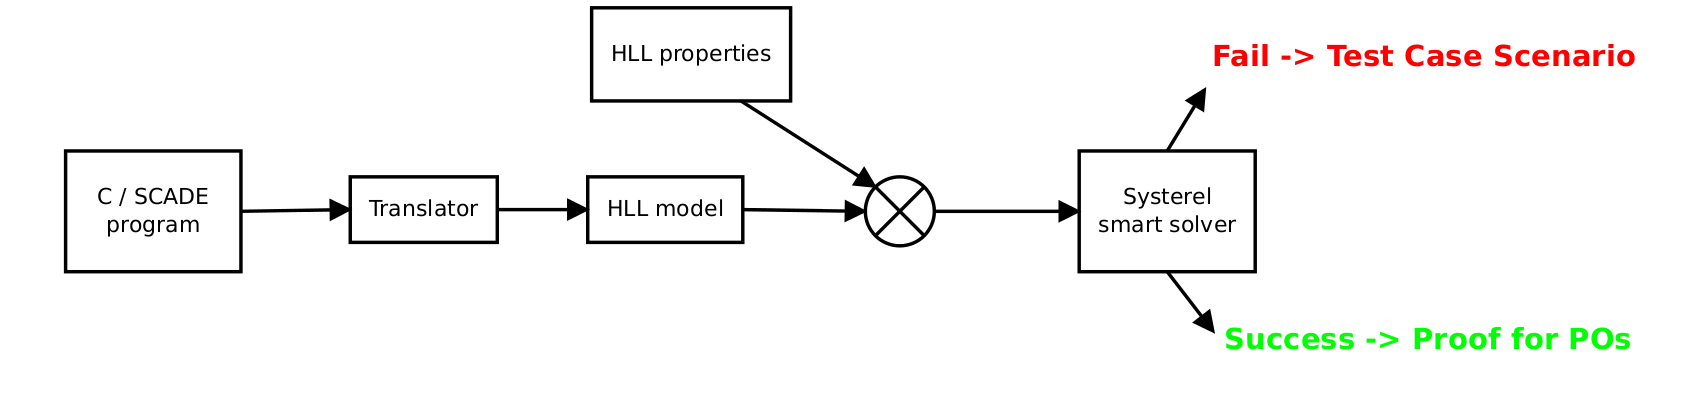
\includegraphics[width=1\textwidth]{S3_process}
\caption{Procedure of verification of Scade model}
\label{fig:procos}
\end{figure}

Figure \ref{fig:procos} describes the process:
\begin{itemize}
\item the main input is a Scade model to  verify (same approach and tool can be applied to a C program) which is translated in a High Level Language (a textual description of the model)
\item the second input is the propreties to verify, written in HLL
\item these both inputs are merged in aunique HLL file, used directly as input of the Systerel Smart Solver (S3 model-checker) for verification
\item result of the S3 tool is Success or Failure; in case of failure counter-example is provided for analyse.
\end{itemize}

The S3 tool is a model-checker which manages as well an internal SATs solver as external SAT solvers.

This process can be apply to cover three purposes:


\paragraph{ Properties of an HLL Model: } The prover may be used to prove or disprove properties of an HLL model. Those properties are modeled as proof obligations.
\begin{figure}[h!]
\centering
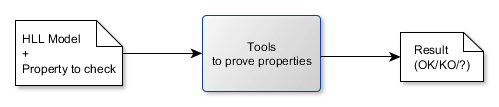
\includegraphics[width=1\textwidth]{Use_property_checker}
\caption{Properties of an HLL Model}
\label{fig:proch}
\end{figure}

\paragraph{ Solving Properties of an HLL Model: } The prover may be used as a solver, by finding values for the streams that comply with some property P. To do so, just put the negation of P as a proof obligation. If the prover succeeds to disprove the proof obligation, it will provide a solution solving P. If the prover succeeds to prove the proof obligation, then this proves that the property cannot be solved.
\begin{figure}[h!]
\centering
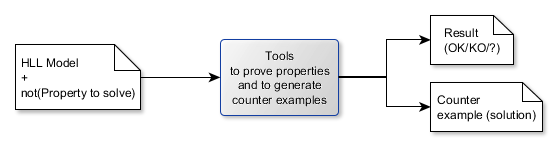
\includegraphics[width=1\textwidth]{Use_property_solver}
\caption{Solving Properties of an HLL Model}
\label{fig:prosolv}
\end{figure}

\paragraph{ Proving the Equivalence of 2 HLL Models: } The prover may be used to prove that 2 HLL models with the same interface (the same input streams and output streams) are equivalent. To do so, an equivalent model is produced with proof obligations stating that for all input streams values, each output of the first HLL model is equal to the output of the second model with the same name.
\begin{figure}[h!]
\centering
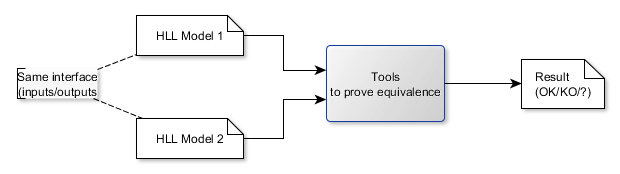
\includegraphics[width=1\textwidth]{Use_equivalence_checker}
\caption{Proving the Equivalence of 2 HLL Models}
\label{fig:eqch}
\end{figure}








\section{Results}

\subsection{Proof of simple properties}

\emph{Conditions to isolate, non-leading, unfitted,...}

\subsection{Verification of use case}

\emph{Start of mission to describe}

\subsection{Comparison of Scade models}

\emph{levels}

\section{Conclusion}


\end{document}